
%\documentclass[11pts,a4paper,amsmath,amssymb,floatfix]{article}%{report}%{book}
\documentclass[12pts,a4paper,amsmath,amssymb,floatfix]{article}%{report}%{book}
\usepackage{graphicx,wrapfig,pdfpages}% Include figure files
%\usepackage{dcolumn,enumerate}% Align table columns on decimal point
\usepackage{enumerate,enumitem}% Align table columns on decimal point
\usepackage{bm,dpfloat}% bold math
\usepackage[pdftex,bookmarks,colorlinks=true,urlcolor=rltblue,citecolor=blue]{hyperref}
\usepackage{amsfonts,amsmath,amssymb,stmaryrd,indentfirst}
\usepackage{times,psfrag}
\usepackage{natbib}
\usepackage{color}
\usepackage{units}
\usepackage{rotating}
\usepackage{multirow}


\usepackage{pifont}
\usepackage{subfigure}
\usepackage{subeqnarray}
\usepackage{ifthen}

\usepackage{supertabular}
\usepackage{moreverb}
\usepackage{listings}
\usepackage{palatino}
%\usepackage{doi}
\usepackage{longtable}
\usepackage{float}
\usepackage{perpage}
\MakeSorted{figure}
%\usepackage{pdflscape}


%\usepackage{booktabs}
%\newcommand{\ra}[1]{\renewcommand{\arraystretch}{#1}}


\definecolor{rltblue}{rgb}{0,0,0.75}


%\usepackage{natbib}
\usepackage{fancyhdr} %%%%
\pagestyle{fancy}%%%%
% with this we ensure that the chapter and section
% headings are in lowercase
%%%%\renewcommand{\chaptermark}[1]{\markboth{#1}{}}
\renewcommand{\sectionmark}[1]{\markright{\thesection\ #1}}
\fancyhf{} %delete the current section for header and footer
\fancyhead[LE,RO]{\bfseries\thepage}
\fancyhead[LO]{\bfseries\rightmark}
\fancyhead[RE]{\bfseries\leftmark}
\renewcommand{\headrulewidth}{0.5pt}
% make space for the rule
\fancypagestyle{plain}{%
\fancyhead{} %get rid of the headers on plain pages
\renewcommand{\headrulewidth}{0pt} % and the line
}

\def\newblock{\hskip .11em plus .33em minus .07em}
\usepackage{color}

%\usepackage{makeidx}
%\makeindex

\setlength\textwidth      {16.cm}
\setlength\textheight     {22.6cm}
\setlength\oddsidemargin  {-0.3cm}
\setlength\evensidemargin {0.3cm}

\setlength\headheight{14.49998pt} 
\setlength\topmargin{0.0cm}
\setlength\headsep{1.cm}
\setlength\footskip{1.cm}
\setlength\parskip{0pt}
\setlength\parindent{0pt}


%%%
%%% Headers and Footers
\lhead[] {\text{\small{EX3029 -- Chemical Thermodynamics}}} 
\rhead[] {{\text{\small{Extra-Examples - Module 06}}}}
%\chead[] {\text{\small{Session 2012/13}}} 
\lfoot[]{Dr Jeff Gomes}
%\cfoot[\thepage]{\thepage}
\rfoot[\text{\small{\thepage}}]{\thepage}
\renewcommand{\headrulewidth}{0.8pt}


%%%
%%% space between lines
%%%
\renewcommand{\baselinestretch}{1.5}

\newenvironment{VarDescription}[1]%
  {\begin{list}{}{\renewcommand{\makelabel}[1]{\textbf{##1:}\hfil}%
    \settowidth{\labelwidth}{\textbf{#1:}}%
    \setlength{\leftmargin}{\labelwidth}\addtolength{\leftmargin}{\labelsep}}}%
  {\end{list}}

%%%%%%%%%%%%%%%%%%%%%%%%%%%%%%%%%%%%%%%%%%%
%%%%%%                              %%%%%%%
%%%%%%      NOTATION SECTION        %%%%%%%
%%%%%%                              %%%%%%%
%%%%%%%%%%%%%%%%%%%%%%%%%%%%%%%%%%%%%%%%%%%

% Text abbreviations.
\newcommand{\ie}{{\em{i.e., }}}
\newcommand{\eg}{{\em{e.g., }}}
\newcommand{\cf}{{\em{cf., }}}
\newcommand{\wrt}{with respect to}
\newcommand{\lhs}{left hand side}
\newcommand{\rhs}{right hand side}
% Commands definining mathematical notation.

% This is for quantities which are physically vectors.
\renewcommand{\vec}[1]{{\mbox{\boldmath$#1$}}}
% Physical rank 2 tensors
\newcommand{\tensor}[1]{\overline{\overline{#1}}}
% This is for vectors formed of the value of a quantity at each node.
\newcommand{\dvec}[1]{\underline{#1}}
% This is for matrices in the discrete system.
\newcommand{\mat}[1]{\mathrm{#1}}


\DeclareMathOperator{\sgn}{sgn}
\newtheorem{thm}{Theorem}[section]
\newtheorem{lemma}[thm]{Lemma}

%\newcommand\qed{\hfill\mbox{$\Box$}}
\newcommand{\re}{{\mathrm{I}\hspace{-0.2em}\mathrm{R}}}
\newcommand{\inner}[2]{\langle#1,#2\rangle}
\renewcommand\leq{\leqslant}
\renewcommand\geq{\geqslant}
\renewcommand\le{\leqslant}
\renewcommand\ge{\geqslant}
\renewcommand\epsilon{\varepsilon}
\newcommand\eps{\varepsilon}
\renewcommand\phi{\varphi}
\newcommand{\bmF}{\vec{F}}
\newcommand{\bmphi}{\vec{\phi}}
\newcommand{\bmn}{\vec{n}}
\newcommand{\bmns}{{\textrm{\scriptsize{\boldmath $n$}}}}
\newcommand{\bmi}{\vec{i}}
\newcommand{\bmj}{\vec{j}}
\newcommand{\bmk}{\vec{k}}
\newcommand{\bmx}{\vec{x}}
\newcommand{\bmu}{\vec{u}}
\newcommand{\bmv}{\vec{v}}
\newcommand{\bmr}{\vec{r}}
\newcommand{\bma}{\vec{a}}
\newcommand{\bmg}{\vec{g}}
\newcommand{\bmU}{\vec{U}}
\newcommand{\bmI}{\vec{I}}
\newcommand{\bmq}{\vec{q}}
\newcommand{\bmT}{\vec{T}}
\newcommand{\bmM}{\vec{M}}
\newcommand{\bmtau}{\vec{\tau}}
\newcommand{\bmOmega}{\vec{\Omega}}
\newcommand{\pp}{\partial}
\newcommand{\kaptens}{\tensor{\kappa}}
\newcommand{\tautens}{\tensor{\tau}}
\newcommand{\sigtens}{\tensor{\sigma}}
\newcommand{\etens}{\tensor{\dot\epsilon}}
\newcommand{\ktens}{\tensor{k}}
\newcommand{\half}{{\textstyle \frac{1}{2}}}
\newcommand{\tote}{E}
\newcommand{\inte}{e}
\newcommand{\strt}{\dot\epsilon}
\newcommand{\modu}{|\bmu|}
% Derivatives
\renewcommand{\d}{\mathrm{d}}
\newcommand{\D}{\mathrm{D}}
\newcommand{\ddx}[2][x]{\frac{\d#2}{\d#1}}
\newcommand{\ddxx}[2][x]{\frac{\d^2#2}{\d#1^2}}
\newcommand{\ddt}[2][t]{\frac{\d#2}{\d#1}}
\newcommand{\ddtt}[2][t]{\frac{\d^2#2}{\d#1^2}}
\newcommand{\ppx}[2][x]{\frac{\partial#2}{\partial#1}}
\newcommand{\ppxx}[2][x]{\frac{\partial^2#2}{\partial#1^2}}
\newcommand{\ppt}[2][t]{\frac{\partial#2}{\partial#1}}
\newcommand{\pptt}[2][t]{\frac{\partial^2#2}{\partial#1^2}}
\newcommand{\DDx}[2][x]{\frac{\D#2}{\D#1}}
\newcommand{\DDxx}[2][x]{\frac{\D^2#2}{\D#1^2}}
\newcommand{\DDt}[2][t]{\frac{\D#2}{\D#1}}
\newcommand{\DDtt}[2][t]{\frac{\D^2#2}{\D#1^2}}
% Norms
\newcommand{\Ltwo}{\ensuremath{L_2} }
% Basis functions
\newcommand{\Qone}{\ensuremath{Q_1} }
\newcommand{\Qtwo}{\ensuremath{Q_2} }
\newcommand{\Qthree}{\ensuremath{Q_3} }
\newcommand{\QN}{\ensuremath{Q_N} }
\newcommand{\Pzero}{\ensuremath{P_0} }
\newcommand{\Pone}{\ensuremath{P_1} }
\newcommand{\Ptwo}{\ensuremath{P_2} }
\newcommand{\Pthree}{\ensuremath{P_3} }
\newcommand{\PN}{\ensuremath{P_N} }
\newcommand{\Poo}{\ensuremath{P_1P_1} }
\newcommand{\PoDGPt}{\ensuremath{P_{-1}P_2} }

\newcommand{\metric}{\tensor{M}}
\newcommand{\configureflag}[1]{\texttt{#1}}

% Units
\newcommand{\m}[1][]{\unit[#1]{m}}
\newcommand{\km}[1][]{\unit[#1]{km}}
\newcommand{\s}[1][]{\unit[#1]{s}}
\newcommand{\invs}[1][]{\unit[#1]{s}\ensuremath{^{-1}}}
\newcommand{\ms}[1][]{\unit[#1]{m\ensuremath{\,}s\ensuremath{^{-1}}}}
\newcommand{\mss}[1][]{\unit[#1]{m\ensuremath{\,}s\ensuremath{^{-2}}}}
\newcommand{\K}[1][]{\unit[#1]{K}}
\newcommand{\PSU}[1][]{\unit[#1]{PSU}}
\newcommand{\Pa}[1][]{\unit[#1]{Pa}}
\newcommand{\kg}[1][]{\unit[#1]{kg}}
\newcommand{\rads}[1][]{\unit[#1]{rad\ensuremath{\,}s\ensuremath{^{-1}}}}
\newcommand{\kgmm}[1][]{\unit[#1]{kg\ensuremath{\,}m\ensuremath{^{-2}}}}
\newcommand{\kgmmm}[1][]{\unit[#1]{kg\ensuremath{\,}m\ensuremath{^{-3}}}}
\newcommand{\Nmm}[1][]{\unit[#1]{N\ensuremath{\,}m\ensuremath{^{-2}}}}

% Dimensionless numbers
\newcommand{\dimensionless}[1]{\mathrm{#1}}
\renewcommand{\Re}{\dimensionless{Re}}
\newcommand{\Ro}{\dimensionless{Ro}}
\newcommand{\Fr}{\dimensionless{Fr}}
\newcommand{\Bu}{\dimensionless{Bu}}
\newcommand{\Ri}{\dimensionless{Ri}}
\renewcommand{\Pr}{\dimensionless{Pr}}
\newcommand{\Pe}{\dimensionless{Pe}}
\newcommand{\Ek}{\dimensionless{Ek}}
\newcommand{\Gr}{\dimensionless{Gr}}
\newcommand{\Ra}{\dimensionless{Ra}}
\newcommand{\Sh}{\dimensionless{Sh}}
\newcommand{\Sc}{\dimensionless{Sc}}


% Journals
\newcommand{\IJHMT}{{\it International Journal of Heat and Mass Transfer}}
\newcommand{\NED}{{\it Nuclear Engineering and Design}}
\newcommand{\ICHMT}{{\it International Communications in Heat and Mass Transfer}}
\newcommand{\NET}{{\it Nuclear Engineering and Technology}}
\newcommand{\HT}{{\it Heat Transfer}}   
\newcommand{\IJHT}{{\it International Journal for Heat Transfer}}

\newcommand{\frc}{\displaystyle\frac}

\newlist{ExList}{enumerate}{1}
\setlist[ExList,1]{label={\bf Example 1.} {\bf \arabic*}}

\newlist{ProbList}{enumerate}{1}
\setlist[ProbList,1]{label={\bf Problem 1.} {\bf \arabic*}}

%%%%%%%%%%%%%%%%%%%%%%%%%%%%%%%%%%%%%%%%%%%
%%%%%%                              %%%%%%%
%%%%%% END OF THE NOTATION SECTION  %%%%%%%
%%%%%%                              %%%%%%%
%%%%%%%%%%%%%%%%%%%%%%%%%%%%%%%%%%%%%%%%%%%


% Cause numbering of subsubsections. 
%\setcounter{secnumdepth}{8}
%\setcounter{tocdepth}{8}

\setcounter{secnumdepth}{4}%
\setcounter{tocdepth}{4}%


\begin{document}



\begin{enumerate}[label=\bfseries Example \arabic*]

%%%
%%% Nguyen (Ex 5.3.1)  
%%%
\item\label{Example:1} Find the bubble point pressure and vapor composition for a liquid mixture of 41.2 mol-$\%$ ethanol (1) and n-hexane (2) at 331 K. Given the Van Laar activity model equations:
\begin{displaymath}
\ln\gamma_{1} = \frc{A}{\left[1+\frc{A x_{1}}{B x_{2}}\right]^{2}}\;\;\;\; \ln\gamma_{2} = \frc{B}{\left[1+\frc{B x_{2}}{A x_{1}}\right]^{2}}\
\end{displaymath}
with A = 2.409 and B = 1.970. Also, the vapour pressure $\left(\text{with } P_{i}^{\text{sat}}\text{ in kPa and } T\text{ in K}\right)$ can be expressed as,
\begin{displaymath}
   \ln P_{1}^{\text{sat}} = 16.1952 - \frc{3423.53}{T-55.7152} \;\;\;\; \ln P_{2}^{\text{sat}} = 14.0568 - \frc{2825.42}{T-42.7089}
\end{displaymath}

\bigskip

{\large{\bf Solution:}}

   \begin{itemize}
      \item At 331 K,  $P_{1}^{\text{sat}}=$ 42.90 kPa and $P_{1}^{\text{sat}}=$ 70.54 kPa.
      \item For the liquid solution with $x_{1}=0.412$ and $x_{2}=1-x_{1}=0.588$, the Van Laar equation,
         \begin{eqnarray}
            \ln\gamma_{1} = \frc{2.409}{\left[1+\frc{2.409 x_{1}}{1.970 x_{2}}\right]^{2}} & \Longrightarrow & \gamma_{1} = 2.0111 \nonumber \\
            \ln\gamma_{2} = \frc{1.790}{\left[1+\frc{1.790 x_{1}}{2.409 x_{1}}\right]^{2}} & \Longrightarrow & \gamma_{2} = 1.5244 \nonumber
         \end{eqnarray}
      \item Partial pressure of ethanol and n-hexane are obtained from,
         \begin{displaymath}
             P_{1} = x_{1}\gamma_{1}P_{1}^{\text{sat}} = 35.55 kPa,\;\;\;P_{2} = x_{2}\gamma_{2}P_{2}^{\text{sat}} = 63.22 kPa
         \end{displaymath}
      \item The bubble point pressure is
         \begin{displaymath}
             {\bf P = P_{1} + P_{2} = 98.77 kPa}
         \end{displaymath}
      \item The composition of the vapour phase is
         \begin{displaymath}
            {\bf y_{1} = \frc{P_{1}}{P} = 0.3599}\;\;\text{ and }\;\; {\bf y_{2} = \frc{P_{2}}{P} = 0.6401}
         \end{displaymath}
   \end{itemize}
\clearpage


%%%
%%% Nguyen (Ex 5.3.2)  
%%%
\item\label{Example:2} Calculate the bubble point temperature and vapor composition for a liquid mixture of 1 mol-$\%$ acetone (1) and water (2) at 101.3 KPa. Given the Wilson activity model:
   \begin{eqnarray}
       &&\ln\gamma_{1} = -\ln\left(x_{1}+x_{2}C_{12}\right) + x_{2}\left(\frc{C_{12}}{x_{1}+x_{2}C_{12}}-\frc{C_{21}}{x_{2}+x_{1}C_{21}}\right) \nonumber \\
       &&\ln\gamma_{2} = -\ln\left(x_{2}+x_{1}C_{21}\right) + x_{1}\left(\frc{C_{21}}{x_{2}+x_{1}C_{21}}-\frc{C_{12}}{x_{1}+x_{2}C_{12}}\right) \nonumber
   \end{eqnarray}
   with $C_{12}=$0.1173 and $C_{21}=$0.4227. Also, the vapour pressure $\left(\text{with } P_{i}^{\text{sat}}\text{ in kPa and } T\text{ in K}\right)$ is given by,
\begin{displaymath}
   \ln P_{1}^{\text{sat}} = 14.71712 - \frc{2975.95}{T-34.5228} \;\;\;\; \ln P_{2}^{\text{sat}} = 16.5362 - \frc{3985.44}{T-38.9974}
\end{displaymath}


\bigskip

{\large{\bf Solution:}}

   \begin{itemize}
      \item Since the vapour mole fractions are unknown, we should start from the main composition constraint, $\sum\limits_{i=1}^{2}y_{i} = 1$.  
      \item Replacing $y_{i}=x_{i}\gamma_{i}P_{1}^{\text{sat}}/P$,
         \begin{displaymath}
            x_{1}\gamma_{1}P_{1}^{\text{sat}} + x_{2}\gamma_{2}P_{2}^{\text{sat}} = P
         \end{displaymath}
      \item For $x_{1} = 0.01$, $x_{2}=0.99$, $C_{12}=$0.1173 and $C_{21}=$0.4227, $\gamma_{1}=$ 13.0695 and $\gamma_{2}=$ 1.0007
      \item With these numerical values, we can replace into the equation above,
         \begin{displaymath}
            (0.01)(13.0695)\exp\left[14.71712 - \frc{2975.95}{T-34.5228}\right] + (0.99)(1.007)\exp\left[16.5362 - \frc{3985.44}{T-38.9974}\right] =  101.3
         \end{displaymath}
         Resulting in {\bf $T=$ 361.71 K} -- the bubble point temperature of this acetone-water mixture.
      \item At this temperature, the saturation pressure of acetone and water are $P_{1}^{\text{sat}}=$ 276.32 kPa and $P_{2}^{\text{sat}}=$ 65.78 kPa, respectively.
      \item The vapour composition is
         \begin{displaymath}
             \mathbf{y_{1} =\frc{x_{1}\gamma_{1}P_{1}^{\text{sat}}}{P} = 0.3565}\;\;\;\text{ and }\;\;\;\; \mathbf{y_{2} = 0.6435}
         \end{displaymath} 
   \end{itemize}
\clearpage

%%%
%%% Nguyen (Ex 5.3.2)  
%%%
\item\label{Example:3} Calculate the dew point temperature and liquid composition for a vapour mixture of 40 mol-$\%$ acetone (1) and water (2) at 101.3 KPa. Use the Wilson model parameters from \ref{Example:2}.


\bigskip

{\large{\bf Solution:}}

   \begin{itemize}
      \item Now, the mole fraction of the liquid phase is unknown, with constraint $\sum\limits_{i=1}^{2} x_{i}=1$, and similar to the previous problem
          \begin{displaymath}
             \sum\limits_{i=1}^{2} = x_{1} + x_{2} = \frc{y_{1}P}{\gamma_{1}P_{1}^{\text{sat}}} +\frc{y_{2}P}{\gamma_{2}P_{2}^{\text{sat}}} = 1  
          \end{displaymath}
      \item However, as the {\bf activity coefficient does depend on the composition of the liquid phase}, we do need to use an iterative method;
      \item As a first estimative, let's assume $x_{1}=0.10$ and $x_{2}=0.90$. Replacing in the Wilson model leads to $\gamma_{1}=5.4291$ and $\gamma_{2}=1.0484$. 
      \item Solving
         \begin{eqnarray}
            && y_{1} + y_{2} = 1 \Longrightarrow \frc{x_{1}\gamma_{1}P_{1}^{\text{sat}}}{P} + \frc{x_{2}\gamma_{2}P_{2}^{\text{sat}}}{P} = 1 \nonumber \\
            && (0.1)(5.4291)\exp\left[14.71712 - \frc{2975.95}{T-34.5228}\right] + (0.9)(1.0484)\exp\left[16.5362 - \frc{3985.44}{T-38.9974}\right] = 101.3
         \end{eqnarray}
      \item  

   \end{itemize}

\end{enumerate} 

%{
%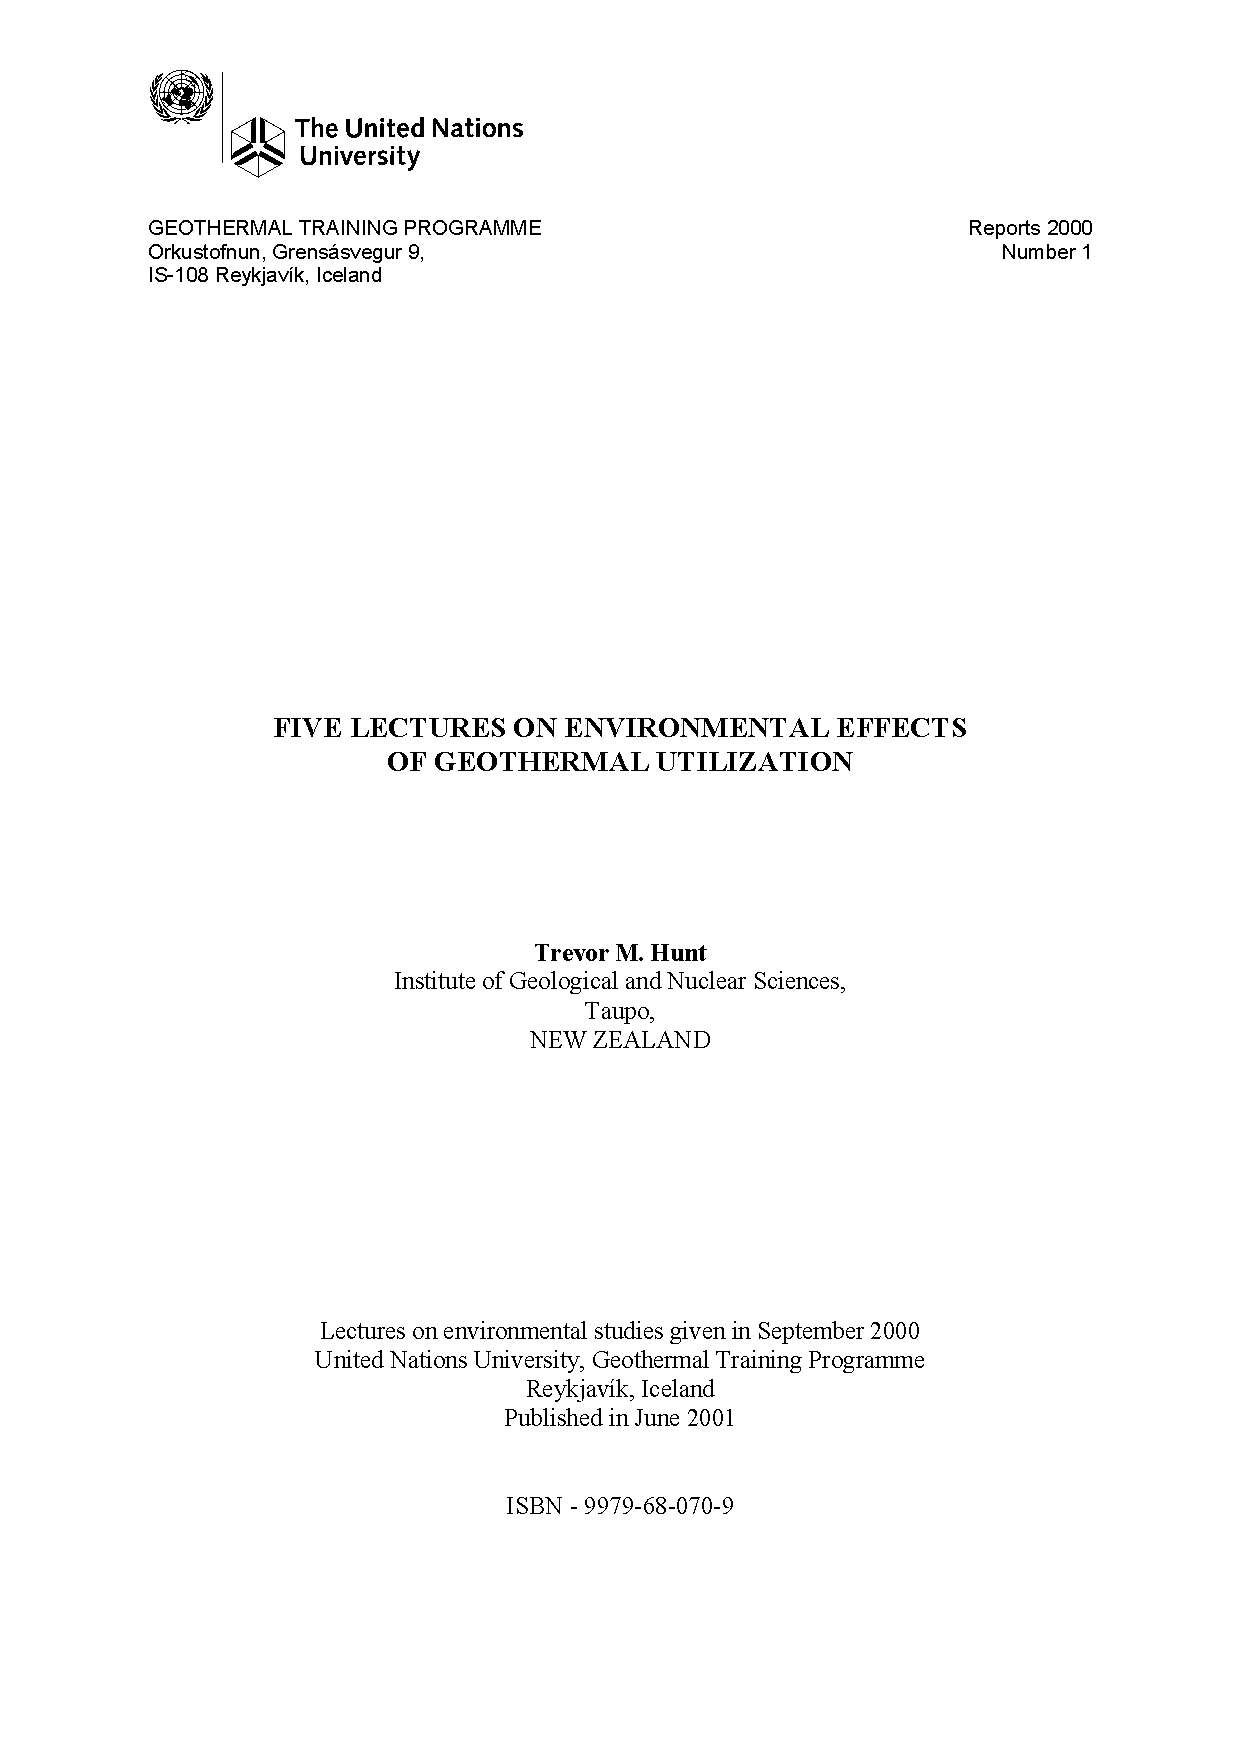
\includepdf[pages=-,fitpaper, angle=0]{./HuntSelect.pdf}
%}

\end{document}
